\section{Gestion de flux de données}
Devant la multiplication des applications à base de flux de données telles que : la gestion des données de capteurs ou la surveillance réseau, les systèmes de gestions de flux de données (\textit{SGFD}) ont étés conçus. L'idée principale de ce type de système étant de permettre une utilisation des flux de données de la même manière que les bases de données. L'interrogation des flux passerait donc par un langage déclaratif (tout comme le \textit{SQL}) avec un grand pouvoir d'expression.
\subsection{Approche des SGFD}
Un flux de données est une série de données qui s'accumule au fur et à mesure du temps. De façon général, il n'est pas supposé une régularité temporelle sur l'arrivée des données dans le flux (tel que \enquote{\it une donnée toutes les 5 secondes}). L'idée de faire une interrogation sur ces flux de données au sens \enquote{gestion de base de données} du terme n'a pas de sens car il y aurait confusion entre les modes d'interrogations continues et instantanées présentés en section~\ref{sec:rw:supervision:criteres:traitement}. En effet, le paradigme des requêtes est fondamentalement différent~\cite{Gurgen:sstreamware}.
\begin{figure}[ht]
    \centering
    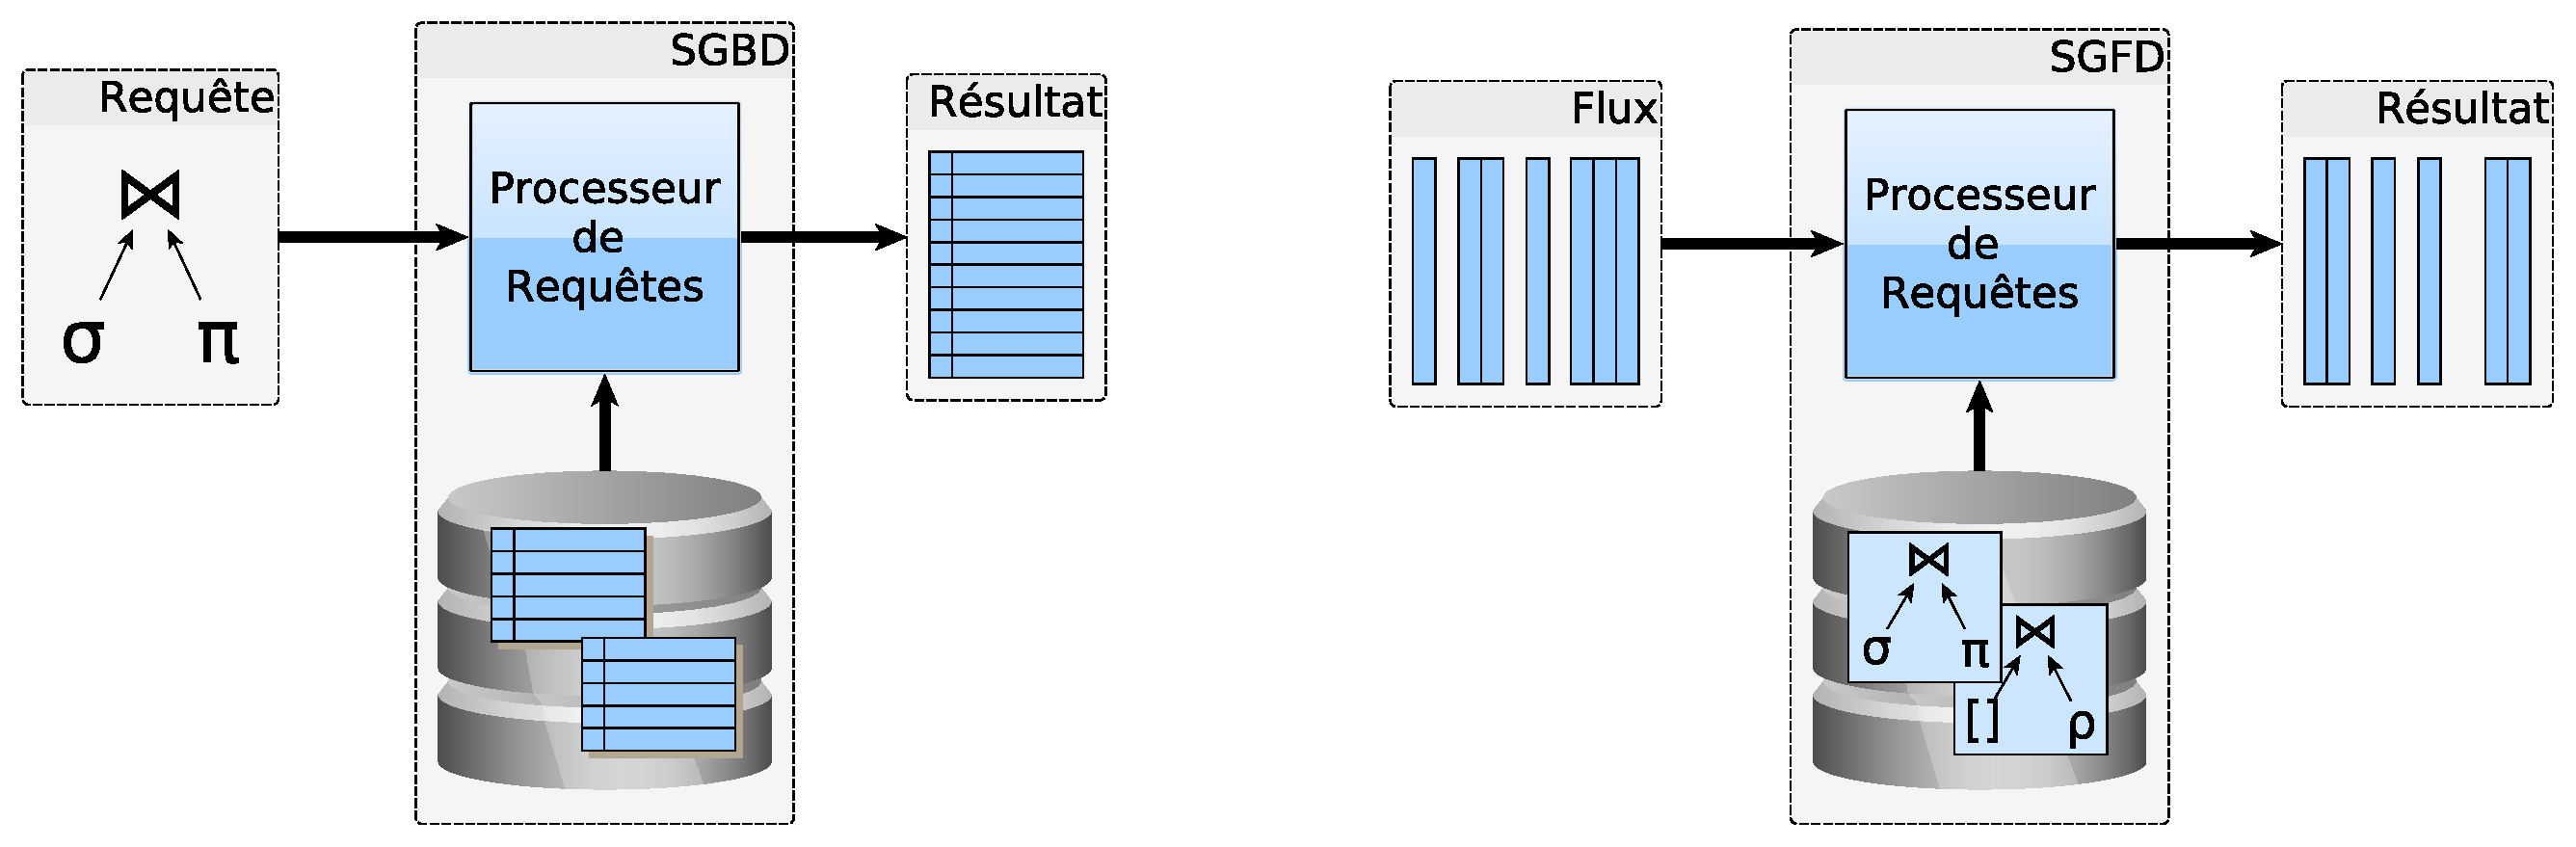
\includegraphics[width=0.75\textwidth]{rw-supervision-sgbd-sgfd}
    \caption{SGBD : Requêtes transitoires, Données persistantes vs SGFD : Données transitoires, Requêtes persistantes}
\end{figure}

\begin{itemize}
    \item[\textbf{Base de données}] : Une requête est une question posée sur un ensemble de relations figées et persistants (principe transactionnel). La réponse est un ensemble de n-uplets. Une fois la requête traitée elle n'existe plus.
    \item[\textbf{Flux de données}] : Une requête un ensemble d'opérateurs et est considéré comme persistant. Le ou les flux de données sont appliqués sur cet ensemble d'opérateurs pour en produire un nouveau flux.
\end{itemize}

\subsection{Principes architecturaux}
\subsection{Les opérateurs}
\subsection{Synthèse}
\begin{table}[!ht]
\criteretabDonnee
    {Modèle dérivé du relationnel mais où le contenu est variable dans le temps.}
    {Pas de structure sémantique en dehors de gestion de méta-données.}
    {Toutes les données sont dynamiques et événementielles a priori.}
\criteretabTraitement
    {Continue.}
    {Il est supposé que chaque source produit un flux de données. Le fait de traiter ces flux participe à l'intégration de sources.}
    {Langages de requêtes similaires aux SQL supportant la dynamique et l'évolution des données}
    {A un instant donné, les opérateurs sont semblables au relationnel. L'expressivité du support du dynamisme reste inconnu encore.}
\criteretabAdaptabilite
    {Création de source pour fournir les flux de données. Comme il n'y a pas de structure sémantique, l'adaptation n'est que l'écriture de requêtes continues.}
    {Pas de perspectives métiers.}
    {Les sources et puits sont en général adaptés par les utilisateurs. Un développement peut être fait dessus, mais il est rarement possible de rajouter des opérateurs.}
    {Très rapide car la latence de traitement doit être contrôlée pour supporter des haut débits.}
\caption{Synthèse des systèmes de gestion de flux de données}\label{tab:rw:supervision:sgfd:synthese}
\end{table}
